\chapter{Jeux d'essais}
\section{Cas de RMBG}
L'utilisation de la combinaison des algorithmes Rate Monotonic et BackGround donne les résultats suivants:
\begin{figure}[htbp]
  \centering
  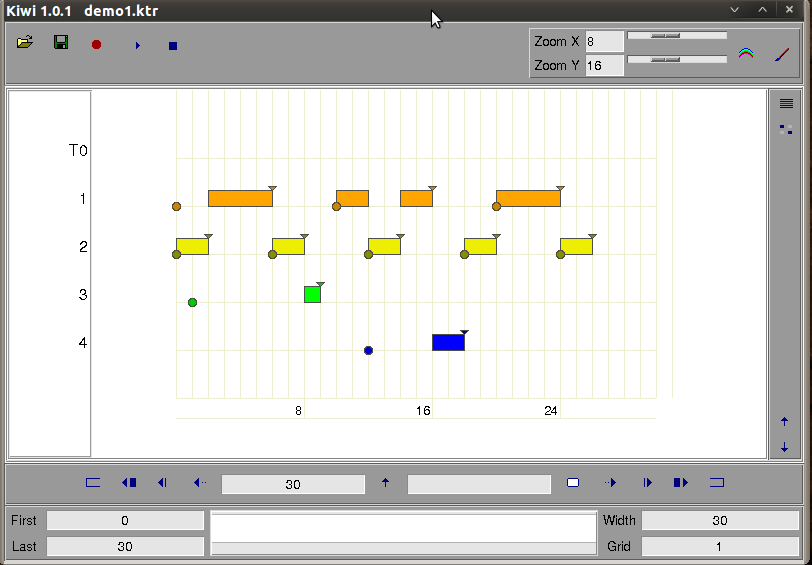
\includegraphics[scale=0.60]{img/RMBG}
  \caption{Résultat de l'appelle à RMBG}
  \label{fig:RMBG}
\end{figure}

\begin{verbatim}
PPCM : 30
Resultat du test de faisabilité : 0.73333335

Déroulement de l'algorithme

****BILAN ET ANALYSE****
Temps d'execution : 30
Temps creux : 5
Utilisation du processeur :83
Nombre de préemptions :1
****TacheAp****
Temps de réponse min : 4
Temps de réponse max : 7
Temps de réponse moy : 6.5
\end{verbatim}
\section{Cas de EDFBG}
L'utilisation de la combinaison des algorithmes Earliest Deadline First et BackGround donne les résultats suivants : 
\begin{figure}[htbp]
  \centering
  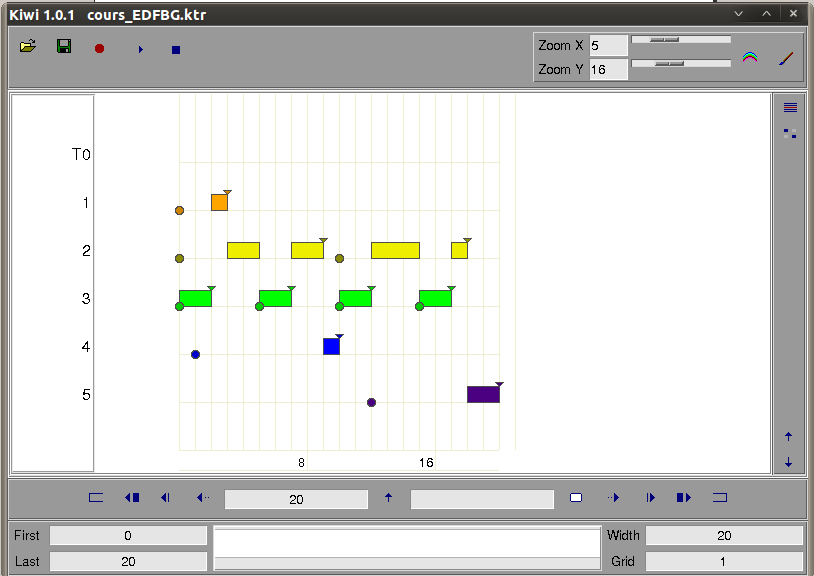
\includegraphics[scale=0.60]{img/EDFBG}
  \caption{Résultat de l'appelle à EDFBG}
  \label{fig:EDFBG}
\end{figure}

\begin{verbatim}
Resutalt du test pour Ci<Pi selon EDF U= : 0
U<=1 condition suffisante vérifiée

Déroulement de l'algorithme

****BILAN ET ANALYSE****
Temps d'execution : 20
Temps creux : 0
Utilisation du processeur :100
Nombre de préemptions :2
****TacheAp****
Temps de réponse min : 6
Temps de réponse max : 8
Temps de réponse moy : 8.0
\end{verbatim}

\section{Cas de EDF-TBS}
L'utilisation de la combinaison des algorithmes Earliest Deadline First et Total Bandwith Server donne les résultats suivants : 
\begin{figure}[htbp]
  \centering
%  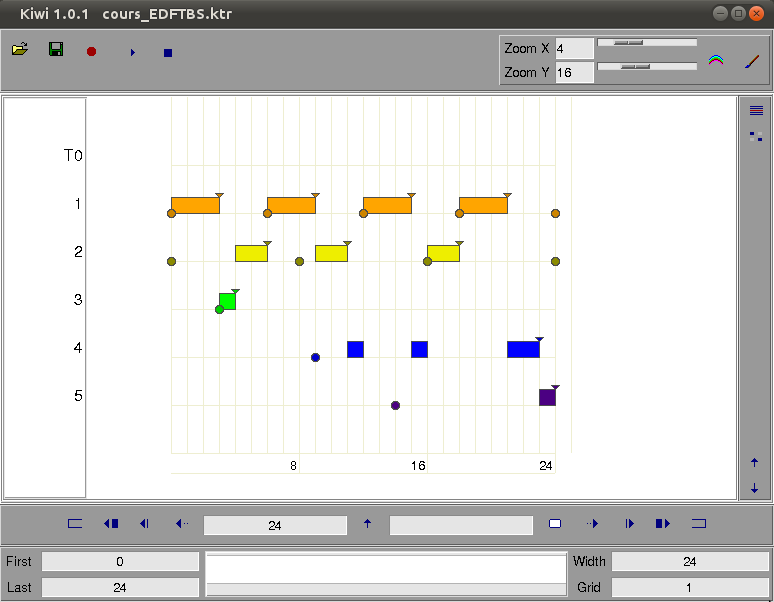
\includegraphics[scale=0.60]{img/EDF-TBS}
  \caption{Résultat de l'appelle à EDF-TBS}
  \label{fig:EDF-TBS}
\end{figure}

\begin{verbatim}

Déroulement de l'algorithme

****BILAN ET ANALYSE****
Temps d'execution : 24
Temps creux : 0
Utilisation du processeur :100
Nombre de préemptions :2
****TacheAp****
Temps de réponse min : 1
Temps de réponse max : 14
Temps de réponse moy : 8.333333
\end{verbatim}

